\documentclass{beamer}%
% Choose how your presentation looks.
%
% For more themes, color themes and font themes, see:
% http://deic.uab.es/~iblanes/beamer_gallery/index_by_theme.html
%
\mode<presentation>
{
  \usetheme{default}      % or try Darmstadt, Madrid, Warsaw, ...
  \usecolortheme{beaver} % or try albatross, beaver, crane, ...
  \usefonttheme{default}  % or try serif, structurebold, ...
  \setbeamertemplate{navigation symbols}{}
  \setbeamertemplate{caption}[numbered]
}

\usepackage[english]{babel}
\usepackage[utf8x]{inputenc}
\usepackage{mathtools}
% \usepackage{blkarray}
\usepackage{tikz}

\newcommand\indx[2]{\genfrac{}{}{0pt}{1}{#1}{#2}}
\newcommand\indxx[2]{(#1,#2)}

\title[Leaf Free]{Counting structures on the $n \times k$ grid graph}
\author{Peter Kagey}
\institute{University of Southern California}
\date[]{
  Graduate Student Combinatorics Conference\\
  April 2019
}

\begin{document}
\begin{frame}
  \titlepage
\end{frame}

% Uncomment these lines for an automatically generated outline.
%\begin{frame}{Outline}
%  \tableofcontents
%\end{frame}

\begin{frame}{Commodore 64} % https://www.youtube.com/watch?v=m9joBLOZVEo
  % When I was working in software, I became known for my one-off programming
  % projects, and so when my colleague ran across this video, he sent it to me,
  % and it indeed piqued my curiosity.
  \center{\includegraphics[width=300pt]{commodore64_1.png}}
\end{frame}

\begin{frame}{Commodore 64} % https://www.youtube.com/watch?v=m9joBLOZVEo
  \center{\includegraphics[width=300pt]{commodore64_2.png}}
\end{frame}

\begin{frame}{Commodore 64} % https://www.youtube.com/watch?v=m9joBLOZVEo
  \center{\includegraphics[width=300pt]{commodore64_3.png}}
\end{frame}

\begin{frame}{Javascript} % https://www.youtube.com/watch?v=m9joBLOZVEo
  \center{\includegraphics[width=300pt]{website_pre.png}}
\end{frame}

\begin{frame}{Javascript} % https://www.youtube.com/watch?v=m9joBLOZVEo
  \center{\includegraphics[width=300pt]{website_post.png}}
\end{frame}

\begin{frame}{Counting grids} % V2 Problem 56.
  \begin{center}
  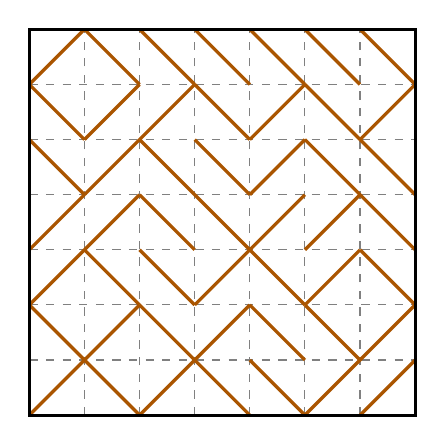
\begin{tikzpicture}[scale=0.7]
    \draw[gray, dashed] (0,0) grid (7,7);
    \foreach \a/\b/\s in {
      0/0/1, 0/1/0, 0/2/1, 0/3/1, 0/4/0, 0/5/0, 0/6/1,
      1/0/0, 1/1/1, 1/2/0, 1/3/1, 1/4/1, 1/5/1, 1/6/0,
      2/0/1, 2/1/0, 2/2/0, 2/3/0, 2/4/0, 2/5/1, 2/6/0,
      3/0/0, 3/1/1, 3/2/1, 3/3/0, 3/4/0, 3/5/0, 3/6/0,
      4/0/0, 4/1/0, 4/2/0, 4/3/1, 4/4/1, 4/5/1, 4/6/0,
      5/0/1, 5/1/0, 5/2/1, 5/3/1, 5/4/0, 5/5/0, 5/6/0,
      6/0/1, 6/1/1, 6/2/0, 6/3/0, 6/4/0, 6/5/1, 6/6/0
    } {
      \draw[very thick, draw={rgb:red,2;green,1;blue,0}] (\a, \b + 1 - \s)--(\a + 1, \b + \s );
    }
    \draw[very thick] (0,0) rectangle (7,7);
  \end{tikzpicture}
  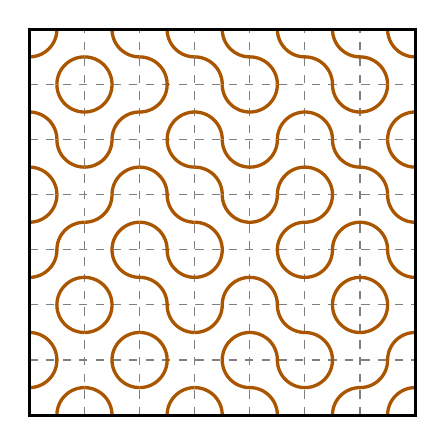
\begin{tikzpicture}[scale=0.7]
    \draw[gray, dashed] (0,0) grid (7,7);
    \foreach \a/\b/\s in {
      0/0/1, 0/1/0, 0/2/1, 0/3/1, 0/4/0, 0/5/0, 0/6/1,
      1/0/0, 1/1/1, 1/2/0, 1/3/1, 1/4/1, 1/5/1, 1/6/0,
      2/0/1, 2/1/0, 2/2/0, 2/3/0, 2/4/0, 2/5/1, 2/6/0,
      3/0/0, 3/1/1, 3/2/1, 3/3/0, 3/4/0, 3/5/0, 3/6/0,
      4/0/0, 4/1/0, 4/2/0, 4/3/1, 4/4/1, 4/5/1, 4/6/0,
      5/0/1, 5/1/0, 5/2/1, 5/3/1, 5/4/0, 5/5/0, 5/6/0,
      6/0/1, 6/1/1, 6/2/0, 6/3/0, 6/4/0, 6/5/1, 6/6/0
    } {
      \draw[very thick, draw={rgb:red,2;green,1;blue,0}, domain=\s*270:\s*270+90]
        plot ({0.5*cos(\x) + \a}, {0.5*sin(\x) + \b + \s});
      \draw[very thick, draw={rgb:red,2;green,1;blue,0}, domain=180-\s*90:270-\s*90]
        plot ({0.5*cos(\x) + \a + 1}, {0.5*sin(\x) + \b  + 1 - \s});
    }
    \draw[very thick] (0,0) rectangle (7,7);
  \end{tikzpicture}
  \end{center}
\end{frame}

\begin{frame}{A295229: Number of tilings of the $n \times n$ grid, using diagonal lines to connect the grid points.}
  % A295229
  \begin{figure}[!h]
  \centering
  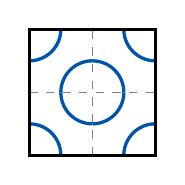
\begin{tikzpicture}[scale=0.8]
    \foreach \a/\b/\theta in {
      0/0/0, 1/1/180,
      1/1/270, 2/0/90,
      0/2/270, 1/1/90,
      1/1/0, 2/2/180} {
      \draw[very thick, draw={rgb:red,0;green,1;blue,2}, domain=\theta:\theta+90] plot ({0.5*cos(\x) + \a}, {0.5*sin(\x) + \b});
    }
    \draw[gray, dashed] (0,0) grid (2,2);
    \draw[very thick] (0,0) rectangle (2,2);
  \end{tikzpicture}
  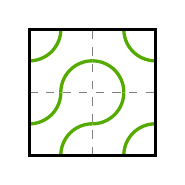
\begin{tikzpicture}[scale=0.8]
    \draw[gray, dashed] (0,0) grid (2,2);
    \foreach \a/\b/\theta in {
      0/1/270, 1/0/90,
      1/1/270, 2/0/90,
      0/2/270, 1/1/90,
      1/1/0, 2/2/180} {
      \draw[very thick, draw={rgb:red,1;green,2;blue,0}, domain=\theta:\theta+90] plot ({0.5*cos(\x) + \a}, {0.5*sin(\x) + \b});
    }
    \draw[very thick] (0,0) rectangle (2,2);
  \end{tikzpicture}
  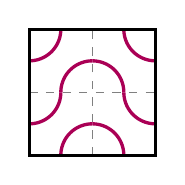
\begin{tikzpicture}[scale=0.8]
    \draw[gray, dashed] (0,0) grid (2,2);
    \foreach \a/\b/\theta in {
      0/1/270, 1/0/90,
      1/0/0, 2/1/180,
      0/2/270, 1/1/90,
      1/1/0, 2/2/180} {
      \draw[very thick, draw={rgb:red,2;green,0;blue,1}, domain=\theta:\theta+90] plot ({0.5*cos(\x) + \a}, {0.5*sin(\x) + \b});
    }
    \draw[very thick] (0,0) rectangle (2,2);
  \end{tikzpicture}
  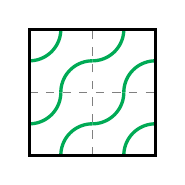
\begin{tikzpicture}[scale=0.8]
    \draw[gray, dashed] (0,0) grid (2,2);
    \foreach \a/\b/\theta in {
      0/1/270, 1/0/90,
      1/1/270, 2/0/90,
      0/2/270, 1/1/90,
      1/2/270, 2/1/90} {
      \draw[very thick, draw={rgb:red,0;green,2;blue,1}, domain=\theta:\theta+90] plot ({0.5*cos(\x) + \a}, {0.5*sin(\x) + \b});
    }
    \draw[very thick] (0,0) rectangle (2,2);
  \end{tikzpicture}
  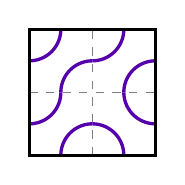
\begin{tikzpicture}[scale=0.8]
    \draw[gray, dashed] (0,0) grid (2,2);
    \foreach \a/\b/\theta in {
      0/1/270, 1/0/90,
      1/0/0, 2/1/180,
      0/2/270, 1/1/90,
      1/2/270, 2/1/90} {
      \draw[very thick, draw={rgb:red,1;green,0;blue,2}, domain=\theta:\theta+90] plot ({0.5*cos(\x) + \a}, {0.5*sin(\x) + \b});
    }
    \draw[very thick] (0,0) rectangle (2,2);
  \end{tikzpicture}
  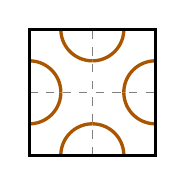
\begin{tikzpicture}[scale=0.8]
    \draw[gray, dashed] (0,0) grid (2,2);
    \foreach \a/\b/\theta in {
      0/1/270, 1/0/90,
      1/0/0, 2/1/180,
      0/1/0, 1/2/180,
      1/2/270, 2/1/90} {
      \draw[very thick, draw={rgb:red,2;green,1;blue,0}, domain=\theta:\theta+90] plot ({0.5*cos(\x) + \a}, {0.5*sin(\x) + \b});
    }
    \draw[very thick] (0,0) rectangle (2,2);
  \end{tikzpicture}
  \\ \vspace{2pt}
  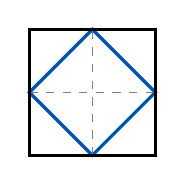
\begin{tikzpicture}[scale=0.8]
    \draw[very thick, draw={rgb:red,0;green,1;blue,2}]
      (0,1)--(1,0)--(2,1)--(1,2)--cycle;
    \draw[gray, dashed] (0,0) grid (2,2);
    \draw[very thick] (0,0) rectangle (2,2);
  \end{tikzpicture}
  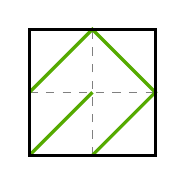
\begin{tikzpicture}[scale=0.8]
    \draw[gray, dashed] (0,0) grid (2,2);
    \draw[very thick, draw={rgb:red,1;green,2;blue,0}]
      (0,0)--(1,1)
      (0,1)--(1,2)--(2,1)--(1,0);
    \draw[very thick] (0,0) rectangle (2,2);
  \end{tikzpicture}
  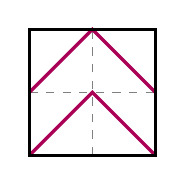
\begin{tikzpicture}[scale=0.8]
    \draw[gray, dashed] (0,0) grid (2,2);
    \draw[very thick, draw={rgb:red,2;green,0;blue,1}]
      (0,0)--(1,1)--(2,0)
      (0,1)--(1,2)--(2,1);
    \draw[very thick] (0,0) rectangle (2,2);
  \end{tikzpicture}
  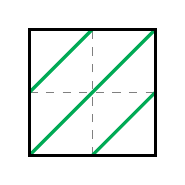
\begin{tikzpicture}[scale=0.8]
    \draw[gray, dashed] (0,0) grid (2,2);
    \draw[very thick, draw={rgb:red,0;green,2;blue,1}]
      (0,1)--(1,2)
      (0,0)--(2,2)
      (1,0)--(2,1);
    \draw[very thick] (0,0) rectangle (2,2);
  \end{tikzpicture}
  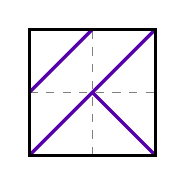
\begin{tikzpicture}[scale=0.8]
    \draw[gray, dashed] (0,0) grid (2,2);
    \draw[very thick, draw={rgb:red,1;green,0;blue,2}]
      (0,1)--(1,2)
      (0,0)--(2,2)
      (1,1)--(2,0);
    \draw[very thick] (0,0) rectangle (2,2);
  \end{tikzpicture}
  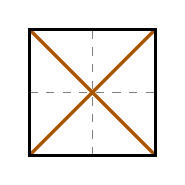
\begin{tikzpicture}[scale=0.8]
    \draw[gray, dashed] (0,0) grid (2,2);
    \draw[very thick, draw={rgb:red,2;green,1;blue,0}]
      (2,0)--(0,2)
      (0,0)--(2,2);
    \draw[very thick] (0,0) rectangle (2,2);
  \end{tikzpicture}
  \caption {
    An example of the $a(2) = 6$ different ways to fill the $2 \times 2$ grid
    with diagonal tiles up to dihedral action of the square.
  }
  \end{figure}
  \[
    a(n) = \begin{cases}
      \frac 18 (2^{n^2} + 2\cdot2^{n(n+1)/2} + 3\cdot2^{n^2/2} + 2\cdot2^{n^2/4}) & n \text{ even} \\
      \frac 18 (2^{n^2} + 2\cdot2^{n(n+1)/2} + 2^{(n^2+1)/2}) & n \text{ odd}
    \end{cases}
  \]
  % $1, 6, 84, 8548, 4203520, 8590557312, 70368815480832, \hdots$
\end{frame}

\begin{frame}{Other tiles} % https://www.youtube.com/watch?v=m9joBLOZVEo
  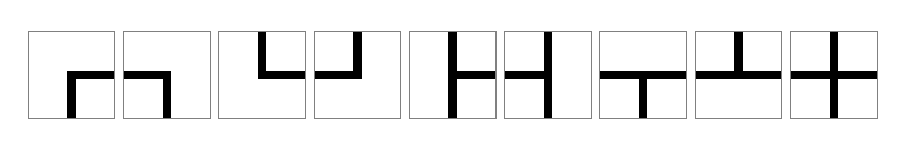
\begin{tikzpicture}[scale=1.1]
    % \draw[gray] (0,0) rectangle (1,1);

    \draw[line width = 3] (2.1,0.5)--(1.6,0.5)--(1.6,0);
    \draw[gray] (1.1,0) rectangle (2.1,1);

    \draw[line width = 3] (2.2,0.5)--(2.7,0.5)--(2.7,0);
    \draw[gray] (2.2,0) rectangle (3.2,1);

    \draw[line width = 3] (3.8,1)--(3.8,0.5)--(4.3,0.5);
    \draw[gray] (3.3,0) rectangle (4.3,1);

    \draw[line width = 3] (4.9,1)--(4.9,0.5)--(4.4,0.5);
    \draw[gray] (4.4,0) rectangle (5.4,1);

    \draw[line width = 3] (6,0)--(6,1) (6,0.5)--(6.5,0.5);
    \draw[gray] (5.5,0) rectangle (6.5,1);

    \draw[line width = 3] (7.1,0)--(7.1,1) (7.1,0.5)--(6.6,0.5);
    \draw[gray] (6.6,0) rectangle (7.6,1);

    \draw[line width = 3] (7.7,0.5)--(8.7,0.5) (8.2,0.5)--(8.2,0);
    \draw[gray] (7.7,0) rectangle (8.7,1);

    \draw[line width = 3] (8.8,0.5)--(9.8,0.5) (9.3,0.5)--(9.3,1);
    \draw[gray] (8.8,0) rectangle (9.8,1);

    \draw[line width = 3] (9.9,0.5)--(10.9,0.5) (10.4,0)--(10.4,1);
    \draw[gray] (9.9,0) rectangle (10.9,1);
  \end{tikzpicture}
  \center{\includegraphics[width=200pt]{pseudomaze.png}}
\end{frame}

\begin{frame}{Baby's first corollary}
  \begin{theorem}[Corollary of Burnside's Lemma]
    Let \begin{itemize}
      \item $t$ be the number of tiles,
      \item $q$ be the number of tiles symmetric under a $90^\circ$ rotation,
      \item $h$ be the number of tiles symmetric under a $180^\circ$ rotation,
      \item $d$ be the number of tiles symmetric under a diagonal reflection, and
      \item $v$ be the number of tiles symmetric under a vertical reflection.
    \end{itemize}
    Then the number of tilings up to symmetries of the square is given by
  \[
    a(n) = \begin{cases}
      \frac 18 (
        t^{n^2} + 2qt^{(n^2-1)/4} + ht^{(n^2-1)/2} + (v^n + d^n)t^{(n^2-n)/2}
      ) & n \text{ odd} \\
      \frac 18 (
        t^{n^2} + 3t^{n^2/2} + 2t^{n^2/4} + 2d^n t^{(n^2-n)/2}
      ) & n \text{ even}
    \end{cases}
  \]
  \end{theorem}
\end{frame}

\begin{frame}{Pipe Mania}
  \center{\includegraphics[width=300pt]{pipe_mania.png}}
\end{frame}

\begin{frame}{Leaf Free Grids} % V2 Problem 56.
  % Can also use this to count multipartite graphs and planar multipartite graphs.
  \begin{figure}[!h]
  \centering
  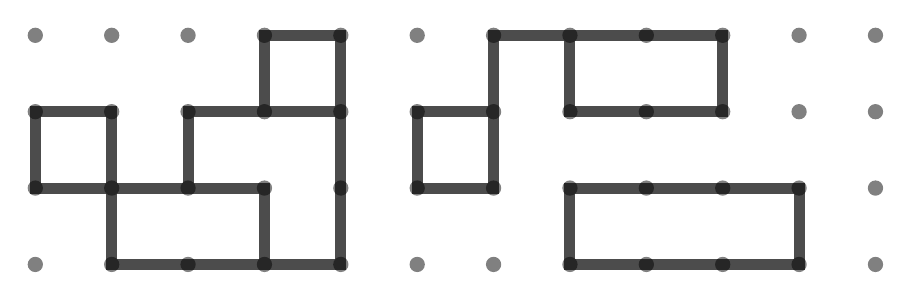
\begin{tikzpicture}[scale=0.97]
    % \draw[very thick, gray, dashed] (0,0) grid (11,3);
    \foreach \i in {0,1,2,3} {
      \foreach \j in {0,1,2,3,4,5,6,7,8,9,10,11} {
        \fill[gray] (\j, \i) circle (0.1);
      }
    }
    \draw[line width=4, opacity=0.7]
      (3,0)--(3,1)--(0,1)--(0,2)--(1,2)--(1,0)--(4,0)--(4,3)--(3,3)--(3,2)--(4,2)
      (2,1)--(2,2)--(3,2)

      (6,2)--(5,2)--(5,1)--(6,1)--(6,2)--(6,3)--(7,3)--(8,3)--(9,3)--(9,2)--(8,2)--(7,2)--(7,3)
      (10,0)--(10,1)--(7,1)--(7,0)--cycle
    ;
  \end{tikzpicture}
  \caption {
    One of the $a_4(12) = 42 650 154 782 713 601$ grids on the $12 \times 4$ grid.
  }
  \end{figure}
  \begin{align*}
    a_2(1) &= 1, a_2(2) = 2 \\
    a_2(n) &= 5a(n-1) - 5a(n-2)
    \\
    \\
    a_3(1) &= 1, a_3(2) = 5, a_3(3) = 43, a_3(4) = 463 \\
    a_3(n) &= 12a(n-1) - 6a(n-2) - 20a(n-3) - 5a(n-4)
    % \\
    % \\
    % a_4(1) &= 1, a_4(2) = 15, a_4(3) = 463, a_4(4) = 16372, \\
    % a_4(5) &= 583199, a_4(6) = 20788249  \\
    % a_4(n) &= 36a_4(n-1) - 7a_4(n-2) - 201a_4(n-3) + 49a_4(n-4) \\
    % &+ 20a_4(n-5) - 5a_4(n-6)
  \end{align*}
\end{frame}

\begin{frame}{Leaf Free Grids: The System of Recurrences}
  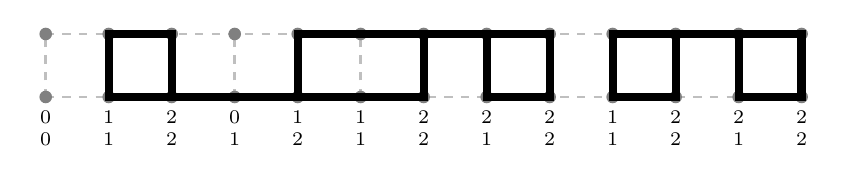
\begin{tikzpicture}[scale=0.8]
  \draw[gray!50, line width=1, dashed] (0,0) grid (12,1);
  \foreach \x in {0, 1, ..., 12} {
    \fill[gray]
      (\x,0) circle (0.1)
      (\x,1) circle (0.1)
    ;
  }
  \draw[line width=3, line cap=round]
    (1,0)--(1,1)--(2,1)--(2,0)--cycle
    (2,0)--(4,0)--(4,1)--(6,1)--(6,0)--(4,0)
    (6,1)--(8,1)--(8,0)--(7,0)--(7,1)
    % (4,1)--(6,1)--(6,0)--(8,0)--(8,1)--(6,1)
    % (2,1)--(4,1)--(4,0)--(2,0)
    % (4,1)--(5,1)--(5,0)--(8,0)--(8,1)--(7,1)--(7,0)
    (9,0) rectangle (10,1)--(11,1) rectangle (12,0);
  ;
  \node at (0,-0.5) {$\indx 00$};
  \node at (1,-0.5) {$\indx 11$};
  \node at (2,-0.5) {$\indx 22$};
  \node at (3,-0.5) {$\indx 01$};
  \node at (4,-0.5) {$\indx 12$};
  \node at (5,-0.5) {$\indx 11$};
  \node at (6,-0.5) {$\indx 22$};
  \node at (7,-0.5) {$\indx 21$};
  \node at (8,-0.5) {$\indx 22$};
  \node at (9,-0.5) {$\indx 11$};
  \node at (10,-0.5) {$\indx 22$};
  \node at (11,-0.5) {$\indx 21$};
  \node at (12,-0.5) {$\indx 22$};
  \end{tikzpicture}
\end{frame}

\begin{frame}{Leaf Free Grids: The System of Recurrences}
  % \begin{tikzpicture}[scale=0.8]
  % \draw[gray!50, line width=1, dashed] (0,0) grid (12,1);
  % \foreach \x in {0, 1, ..., 12} {
  %   \fill[gray]
  %     (\x,0) circle (0.1)
  %     (\x,1) circle (0.1)
  %   ;
  % }
  % \draw[line width=3, line cap=round]
  %   (1,0)--(1,1)--(2,1)--(2,0)--cycle
  %   (2,0)--(4,0)--(4,1)--(6,1)--(6,0)--(4,0)
  %   (6,1)--(8,1)--(8,0)--(7,0)--(7,1)
  %   % (4,1)--(6,1)--(6,0)--(8,0)--(8,1)--(6,1)
  %   % (2,1)--(4,1)--(4,0)--(2,0)
  %   % (4,1)--(5,1)--(5,0)--(8,0)--(8,1)--(7,1)--(7,0)
  %   (9,0) rectangle (10,1)--(11,1) rectangle (12,0);
  % ;
  % \node at (0,-0.5) {$\indx 00$};
  % \node at (1,-0.5) {$\indx 11$};
  % \node at (2,-0.5) {$\indx 22$};
  % \node at (3,-0.5) {$\indx 01$};
  % \node at (4,-0.5) {$\indx 12$};
  % \node at (5,-0.5) {$\indx 11$};
  % \node at (6,-0.5) {$\indx 22$};
  % \node at (7,-0.5) {$\indx 21$};
  % \node at (8,-0.5) {$\indx 22$};
  % \node at (9,-0.5) {$\indx 11$};
  % \node at (10,-0.5) {$\indx 22$};
  % \node at (11,-0.5) {$\indx 21$};
  % \node at (12,-0.5) {$\indx 22$};
  % \end{tikzpicture}
  \begin{align*}
    a_{\indxx 00}(n) &= a_{\indxx 00}(n - 1) + a_{\indxx 22}(n - 1) \\
    a_{\indxx 10}(n) &= a_{\indxx 00}(n - 1) + a_{\indxx 22}(n - 1)
  \end{align*}
\end{frame}

\begin{frame}{System of Recurrences: Getting one long recurrence}
  % \[
    % \begin{bmatrix}
      % a_{11} & a_{12} & \hdots & a_{1k} \\
  %     a_{21} & a_{22} & \hdots & a_{2k} \\
  %     \cdots & \cdots & \ddots & \cdots \\
  %     a_{k1} & a_{k2} & \hdots & a_{kk} \\
  %   \end{bmatrix}^n
  %   \bmatrix{}
  % \]
\end{frame}

\begin{frame}{Mazes and Spanning Trees}
\end{frame}

\begin{frame}{Systems of linear equations}
\end{frame}

\begin{frame}{Generalizations}
\end{frame}


\end{document}
